% annexes
\label{annexe_distribution_0_9}

%{\large R\'esultats de la modification de $k \in \{1,2,3,4,5\}$ cases avec $p=0.5$ }
\begin{figure}[htb!] 
\centering
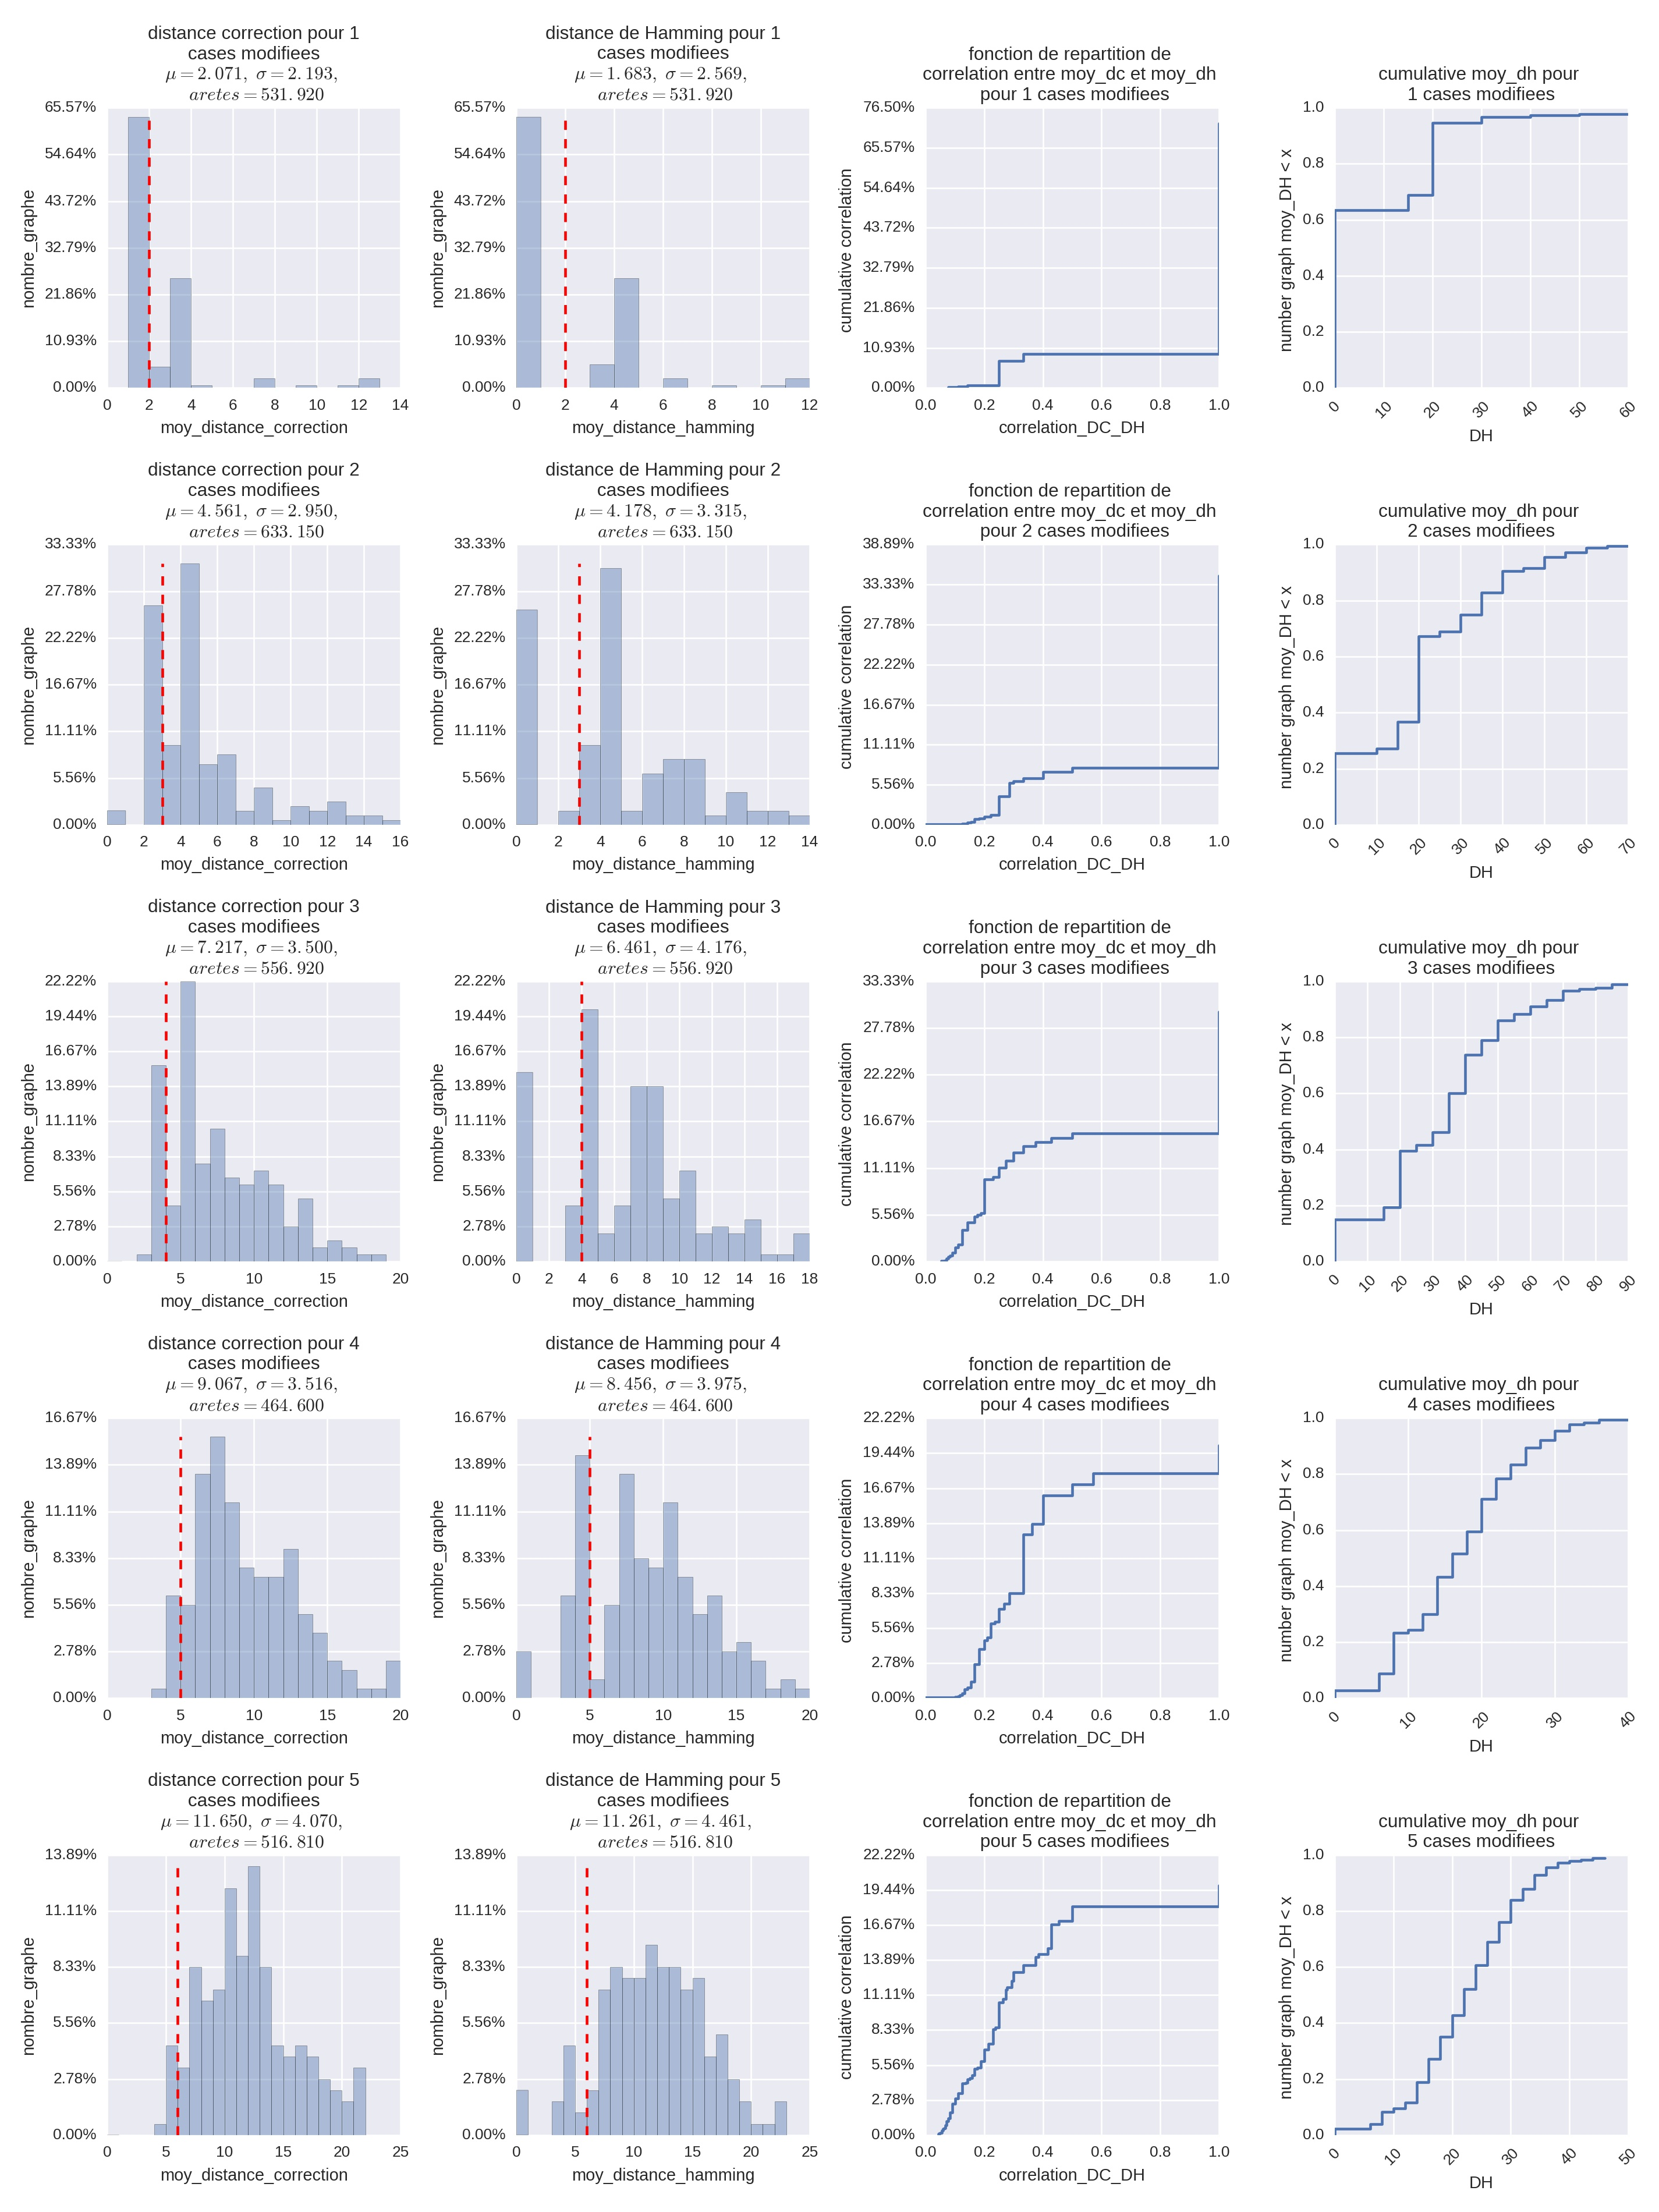
\includegraphics[width=550pt,height=580pt]{unitaire_aleatoire_sansRemise_distanceMoyenDLDH_k_1_2_3_4_5_p_05.jpeg}
\caption{ Approche de correction al\'eatoire sans remise \`a co\^ut unitaire pour $k =\{1,2,3,4,5\} $ cases modifi\'ees : La premi\`ere colonne repr\'esente la distribution des distances de correction $moy\_DC_{k,0.5}$. La seconde colonne est la distribution des distances de Hamming $moy\_DH_{k,0.5}$. La troisi\`eme colonne  est la fonction de repartition de la corr\'elation entre les distances de correction et de Hamming avec en abscisse la corr\'elation entre ces distances (correlation\_DC\_DH).  La quatri\`eme colonne est la fonction cumulative des distances de Hamming. La premi\`ere ligne est associ\'ee \`a $k=1$ case modifi\'ee, la seconde ligne \`a $k=2$ cases modifi\'ees, la troisi\`eme ligne \`a $5$ cases modifi\'ees et enfin la derni\`ere \`a $9$ cases modifi\'ees.}
\label{sansremise_unitaire_distanceMoyenDCDH_k_1_5_aleatoire_p_05} 
\end{figure}
\FloatBarrier

%{\large R\'esultats de la modification de $k \in \{6,7,8,9,\}$ cases avec $p=0.5$ }
\begin{figure}[htb!] 
\centering
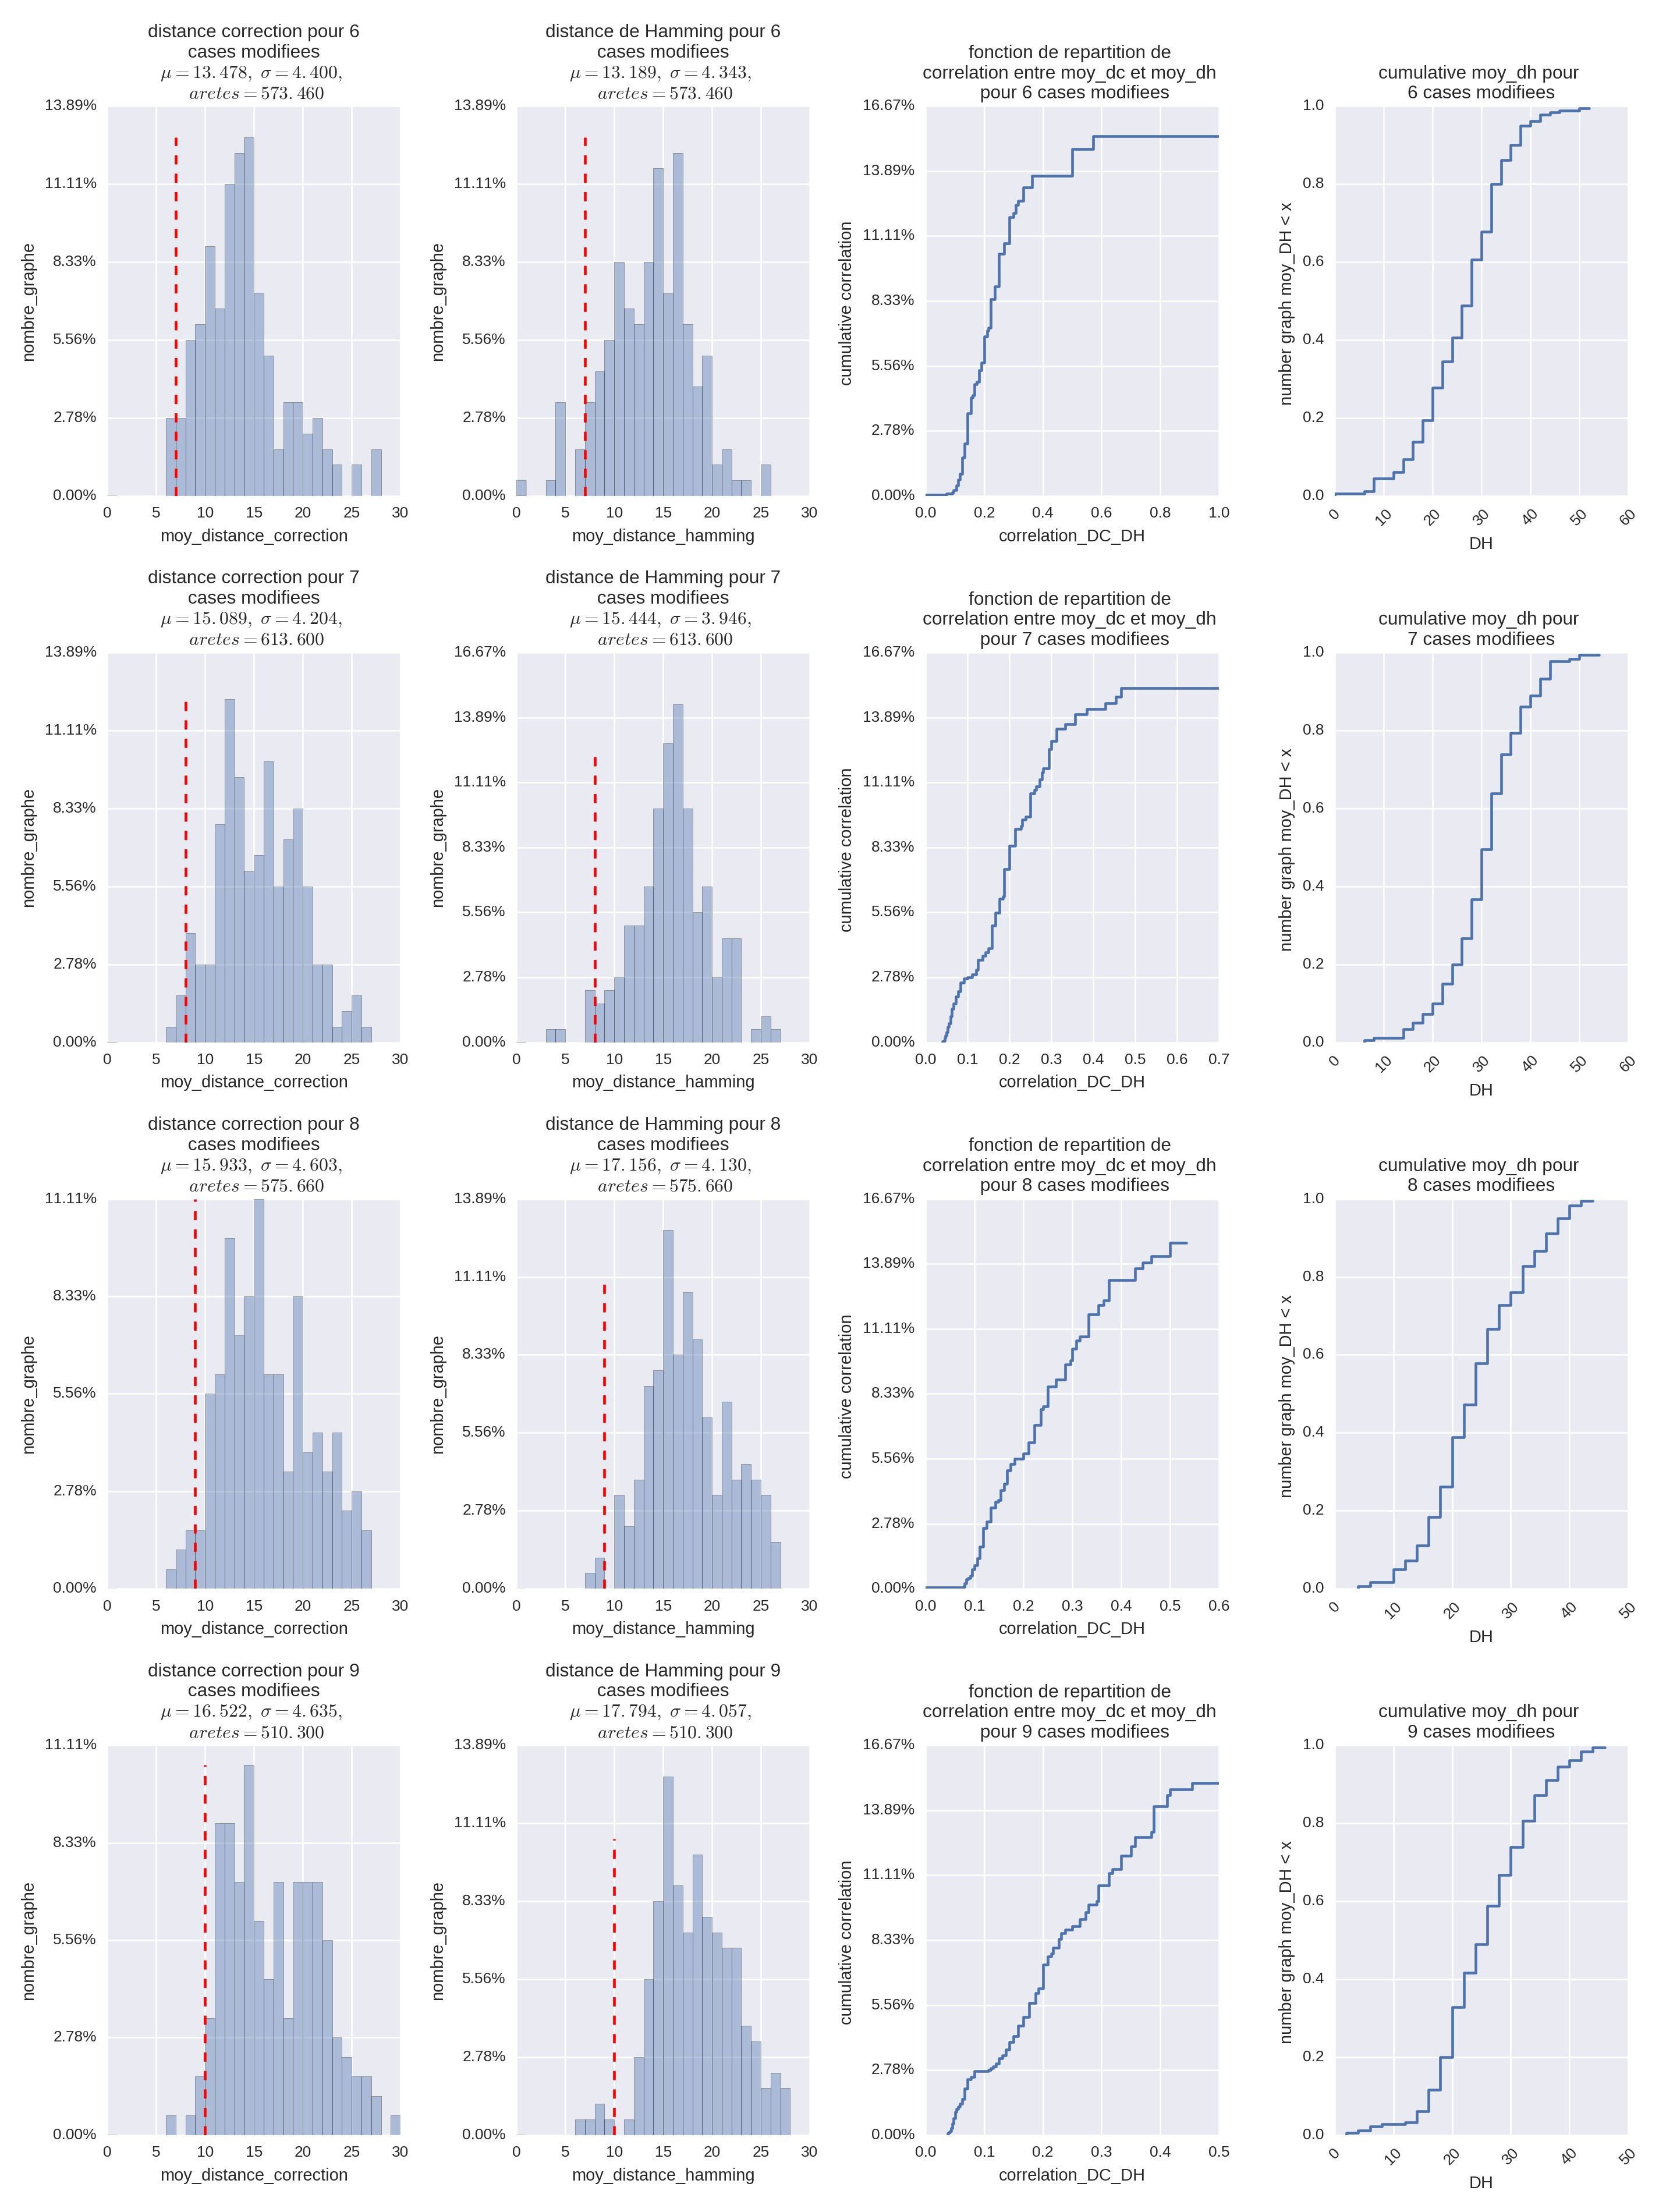
\includegraphics[width=550pt,height=580pt]{unitaire_aleatoire_sansRemise_distanceMoyenDLDH_k_6_7_8_9_p_05.jpeg}
\caption{ Approche de correction al\'eatoire sans remise \`a co\^ut unitaire pour $k =\{6,7,8,9\} $ cases modifi\'ees : La premi\`ere colonne repr\'esente la distribution des distances de correction $moy\_DC_{k,0.5}$. La seconde colonne est la distribution des distances de Hamming $moy\_DH_{k,0.5}$. La troisi\`eme colonne  est la fonction de repartition de la corr\'elation entre les distances de correction et de Hamming avec en abscisse la corr\'elation entre ces distances (correlation\_DL\_DH).  La quatri\`eme colonne est la fonction cumulative des distances de Hamming. La premi\`ere ligne est associ\'ee \`a $k=1$ case modifi\'ee, la seconde ligne \`a $k=2$ cases modifi\'ees, la troisi\`eme ligne \`a $5$ cases modifi\'ees et enfin la derni\`ere \`a $9$ cases modifi\'ees.}
\label{sansremise_unitaire_distanceMoyenDCDH_k_6_9_aleatoire_p_05} 
\end{figure}

